\section{Tilting mechanism}\label{sec:const:tilt}

\begin{enumerate}
  \item Requirements
  \subitem Angular range
\end{enumerate}

%\subsubsection*{Concept}

The tilting mechanism should allow the PCBs to tilt around two axis. For developing the concept the PCBs are displayed as a plane. Figure \ref{fig:const:tilt:mech} and \ref{fig:const:tilt:math} show the front and top view of the tilting mechanism for one axis.\p
%
The PCBs are hold in place by a joint in the center of the plane (\textbf{A}). Now if the top of the PCBs is moved forwards or backwards (\textbf{B}), the plane rotates. The forward and backward movement can be created by connecting to shafts (\textbf{D} and \textbf{E}) with a joint. The base of \textbf{D} is fixed (\textbf{F}) while the end of \textbf{E} is connected to the top of the plane. This creates the triangle \textbf{D} - \textbf{E} - \textbf{B}. When the base of \textbf{D} is now rotated the shape of the triangle is changed, increasing or decreasing the length of \textbf{B}.
The rotation around two axis can be achieved by adding a second \textbf{D} - \textbf{E} - \textbf{B} triangle to the left or right side of the plane.
%
\begin{figure}
  \begin{subfigure}[b]{0.49\textwidth}
    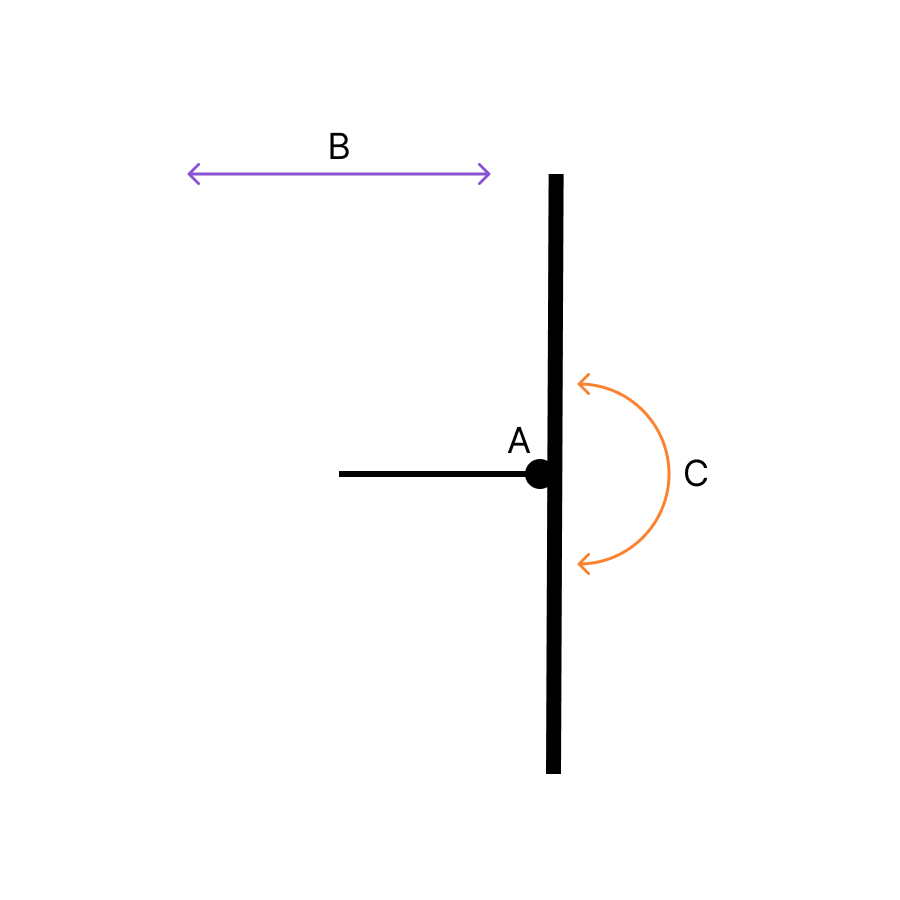
\includegraphics[width=\textwidth]{src/assets/pictures/construction/mec_front.png}
    \caption{Front view}
    \label{fig:const:tilt:mech_front}
  \end{subfigure}
  \hfill
  \begin{subfigure}[b]{0.49\textwidth}
    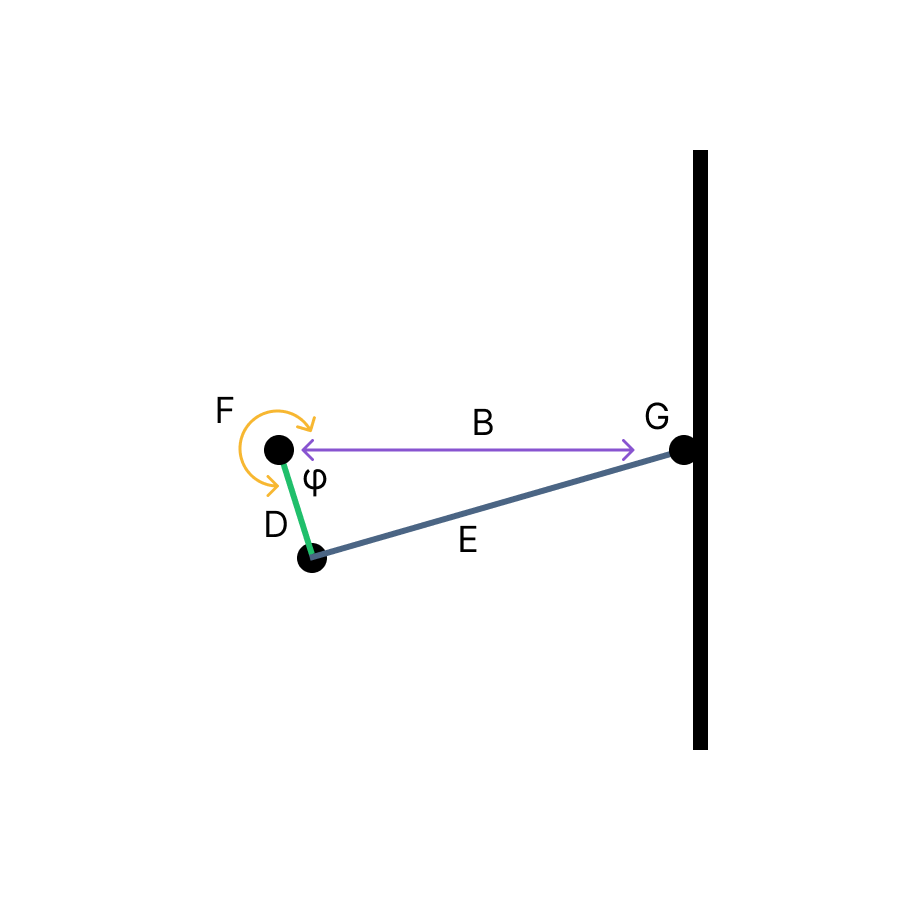
\includegraphics[width=\textwidth]{src/assets/pictures/construction/mec_top.png}
    \caption{Top view}
    \label{fig:const:tilt:mech_top}
  \end{subfigure}
  \caption{Mechanical sketch of the tilting mechanism}
  \label{fig:const:tilt:mech}
\end{figure}
%
\begin{figure}
  \begin{subfigure}[b]{0.49\textwidth}
    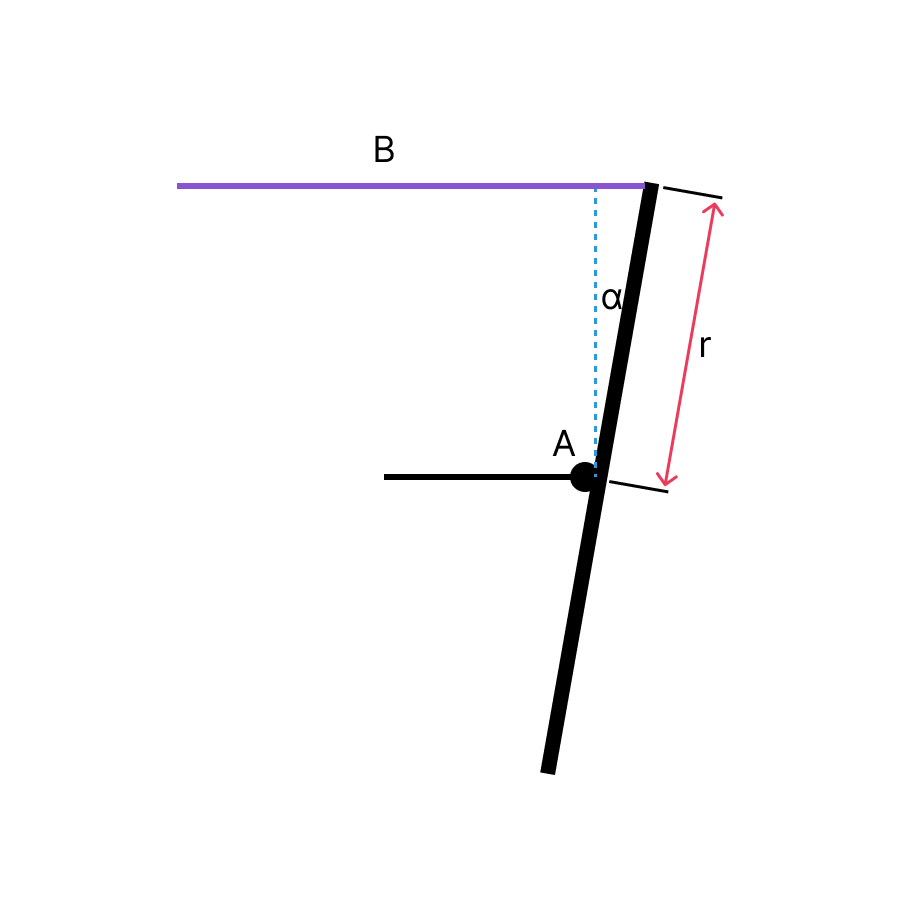
\includegraphics[width=\textwidth]{src/assets/pictures/construction/math_front.png}
    \caption{Front view}
    \label{fig:const:tilt:math_front}
  \end{subfigure}
  \hfill
  \begin{subfigure}[b]{0.49\textwidth}
    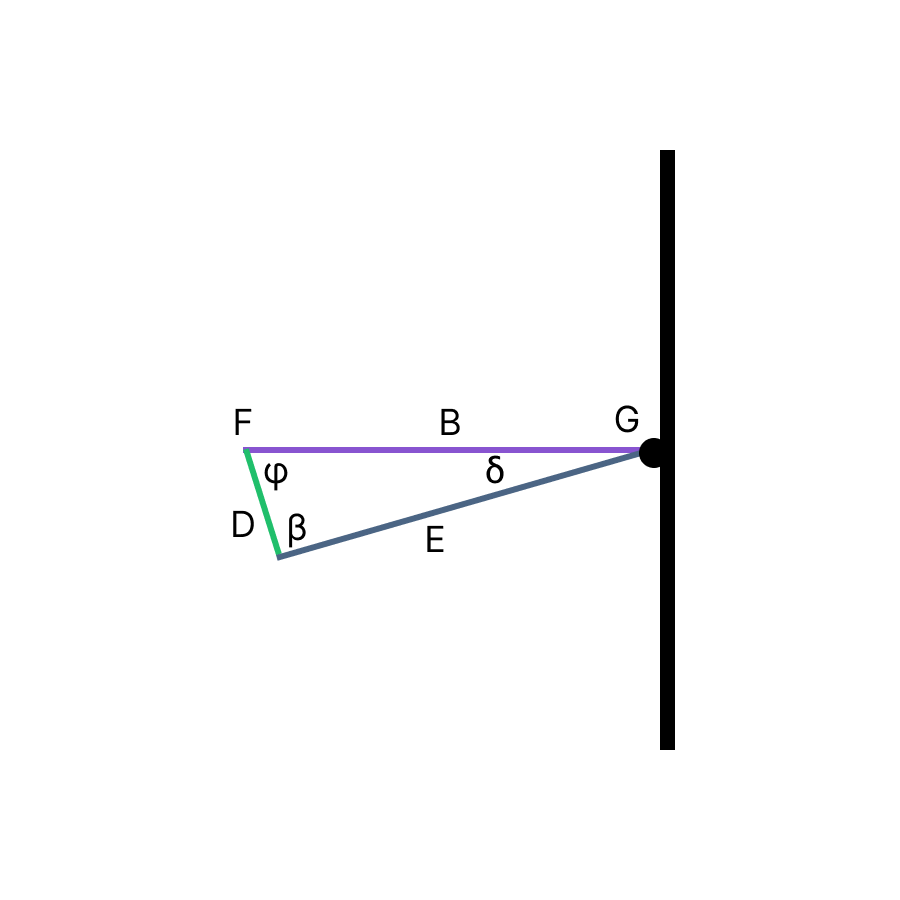
\includegraphics[width=\textwidth]{src/assets/pictures/construction/math_top.png}
    \caption{Top view}
    \label{fig:const:tilt:math_top}
  \end{subfigure}
  \caption{Mathematical sketch of the tilting mechanism}
  \label{fig:const:tilt:math}
\end{figure}
\p
Using this setup the tilting angle $\alpha$ is controlled using the angle $\varphi$. This can be described mathematically as follows. First $\varphi$ is defined with the length of \textbf{B} using the law of cosines.
%
\begin{align}
  E^2     &= D^2 + B^2 - 2DE \cdot \cos \varphi \pmath
  \varphi &= \arccos \left( \frac{D^2 + B^2 - E^2}{2DE} \right) \label{eq:const:tilt:phi_semi}
\end{align}
%
Next $\alpha$ is used to describe \textbf{B}. The result is inserted into equation \ref{eq:const:tilt:phi_semi}.
%
\begin{align}
  \sin \alpha &= \frac{B - B_0}{r}\pmath
  B           &= \sin (\alpha) \cdot r + B_0\pmath
  \mathrm{with~} B_0 &= B(\alpha = 0^\circ, \varphi = 90^\circ) = \sqrt{D^2 + E^2}\pmath
  B           &= \sin (\alpha) \cdot r + \sqrt{D^2 + E^2}
\end{align}
%
\textbf{B$_0$} is the length of \textbf{B} when $\alpha = 0^\circ$. To achieve symmetric movement $\alpha$ is defined to be $0^\circ$ when $\varphi = 90^\circ$. This results in the following equation for $\varphi$:
%
\begin{align}
  \varphi &= \arccos \left( \frac{D^2 + (\sin (\alpha) \cdot r + \sqrt{D^2 + E^2})^2 - E^2}{2DE} \right)
\end{align}
%
It should be noted that this solution is only an approximation. As shown in figure \ref{fig:const:tilt:math} even though the plane rotates, \textbf{B} remains in a straight line. In reality the plane would rotate on a circular path which would change the angle of \textbf{B} (in the front view) and with it the actual length of \textbf{B} debending on the angle $\alpha$. However during testing on the real speaker the error of the calculation wasn't noticeable.